%************************************************
\chapter{The Substrate for Accountable Layered Systems}
\label{chapter:the_substrate_for_accountable_layered_systems}
%************************************************

%\newcommand{\FibR}{$\text{Fib}^\text{R }$}
%\newcommand{\SALS}{SALS}

My implementation is based on a virtual machine that allows parallel
and concurrent scheduling of Lisp-like programs.  I refer to this
virtual machine as \emph{SALS}, the substrate for accountable layered
systems, the focus of this dissertation.  The purpose of SALS is to
provide a simulation of the actual dynamic qualities of Duration, the
activities in Duration that actually exist.  I have previously
explained why computers cannot create meaningful symbolic references
to reality, beyond the purely tautological, in
\autoref{section:digital_reflection}.  If this simulation creates
symbols, they are only in the eyes of the beholder.

In this dissertation, I am focusing on how SALS demonstrates
reflective learning in two distinct causal classes of knowledge from a
single physical expectation failure.  I must begin my description with
the dynamic activities in Duration.  Thus, first, I will describe how
SALS simulates the activities in Duration.  I will explain the
symbolization of these activities in the context of a block building
physical simulation.  I will describe how causal models are learned.
I will give examples of how causal models are put together into plan
objects that are simple serial and parallel SALS programs.  I will
explain how a plan may begin executing and fail.  Finally, I will
describe how the expectation failure response updates causal models in
both reflective layers.  This, in total, shows how learning how to
plan is simulated by SALS.

\section{Fibers Simulate Activities}

SALS introduces an object that represents a parallel process, the
\emph{fiber}.  Fibers are the fundamental element for simulating
concurrent activity in SALS.  SALS begins the simulation with only
one fiber that serves a predefined ``boot-up'' function that starts
all of the other concurrent fibers that are necessary for simulating
the mind.  Fibers are the discrete elements that I have used as a
model of the concurrent, actually inseparable, activities in Duration.

My simulation of mind uses hundreds of thousands of fibers in order to
demonstrate two layers of reflective learning.  Fibers are often very
short-lived processes; for example, not execution, but simply
compiling a single Lisp-like expression in SALS can lead to the
creation and destruction of hundreds of fibers of activity.  Fibers
are generally useful in programs that could use an extra perspective
on a problem.

\section{Symbols and Simulated Symbols}

It becomes important at this point to keep track of the layer of
artificiality that results when one simulates thinking.  The danger is
in losing an awareness of the difference between what one is thinking
and what a simulation is simulating as thought.  For example, a
programmer types symbols to express commands to the computer in a
programming language.  These symbols have meaning to the programmer.
The computer continually repeats the same symbolic manipulation
function, the combinational device.  So, when the simulation appears
to create new symbols by manipulating the symbols contained within its
programming, this is an illusion.  The observer of output from the
simulation may create new symbols, but the machine only has meaning in
terms of the symbols of its programming.

Therefore, I will use an asterisk notation for referring to different
classes of simulated artificiality.  For example, I will continue to
use, simply, the term symbol to refer to the symbols that are actually
reflectively symbolized in order to refer to the activities in
Duration.  These are the symbols that the programmer uses to refer to
the activities of Duration, which gives meaning to the program.  The
programmer then writes a program that simulates the symbolization of
simulated activities in Duration.  When I am referring to the
simulation of the process of symbolization, I will refer to this as a
simulated symbol, or a \emph{symbol*}.  A symbol* is a spatial
arrangement of symbols that have been provided in the programming of
the machine.  I will refer to the creation of this Spatial arrangement
as the creation of a symbol*.

Now that I have described the difference between the symbols the
programmer types and the symbols* that the AI simulates as being
created, the first goal of my description of the implementation is to
describe how SALS simulates the creation of a symbol.  The rest of
this chapter will cover the creation of a symbol*, but first, I must
discuss how the activities in Duration begin simulating by programming
lists of symbols into SALS' interactive programming language.

\section{Programming Language}

SALS includes a Lisp-like programming language, which is programmed
by typing statements that are called \emph{expressions}.  If
expression \ref{expression:print_hello} were typed into SALS, the
symbol ``green'' would be printed to the user's terminal screen.
\begin{equation}
\label{expression:print_hello}
\text{\tt [print `green]}
\end{equation}
The {\tt print} command is a useful debugging tool that can report
status messages to the programmer as the fiber reaches a specific
point in the program.

\section{Sequential and Parallel Programs}

SALS includes expressions for describing serial and parallel
programs.  For example, the expression
\begin{equation*}
\begin{array}{l}
\text{\tt [prog [print 1]} \\
\text{\tt ~~~~~~[print 2]} \\
\text{\tt ~~~~~~[print 3]]}
\end{array}
\end{equation*}
results in the output trace
\begin{equation*}
\begin{array}{l}
\text{\tt 1} \\
\text{\tt 2} \\
\text{\tt 3.}
\end{array}
\end{equation*}
The command {\tt prog} is a way for expressing a sequence of commands
to be executed in serial order.  SALS also includes the {\tt parog}
command for executing a list of commands in parallel, waiting for them
all to complete, and then continuing.
\begin{equation*}
\begin{array}{l}
\text{\tt [parog [print 1]} \\
\text{\tt ~~~~~~~[print 2]} \\
\text{\tt ~~~~~~~[print 3]]}
\end{array}
\end{equation*}
When {\tt parog} is used, it is unclear what command will complete
first because they are all running concurrently, in parallel, starting
at slightly different times.  Here is an example output trace from the
{\tt parog} expression:
\begin{equation*}
\begin{array}{l}
\text{\tt 3} \\
\text{\tt 1} \\
\text{\tt 2.}
\end{array}
\end{equation*}
The {\tt parog} expression is one way to easily start a number of
parallel fibers to simultaneously execute a number of different tasks
and wait for these tasks to complete.

\section{Fibers Create Objects}

SALS includes an object type system.  Every expression in SALS,
besides {\tt nil}, has an object type.  Objects in SALS are in most
cases based on a frame knowledge representation.  Objects have three
main classes of functionality: {\tt get}, {\tt set}, and {\tt have}.
The meaningful uses of these types of functionality are as follows:
\begin{itemize}
\item {\tt [get <object> <slot-name>]}

The object-oriented {\tt get} command retrieves the value from the
named slot of the object's frame.
\item {\tt [set <object> <slot-name> <new-value>]}

The object-oriented {\tt set} command mutates the value at the named
slot of the object's frame to be the given new value.
\item {\tt [have <object> <slot-name> <arguments>]}

The object-oriented {\tt have} command performs other types of
activities that are not simple frame slot accessors and mutators.  The
{\tt have} commands sometimes involve complex mutations or other
side-effects.
\end{itemize}




\section{Creating Parallel Fibers}

The {\tt apply} operator is the normal way for a SALS program to
evaluate a given function with arguments:
\begin{equation*}
\text{\tt [apply <function> <arguments>]}
\end{equation*}
The fundamental operator of SALS's parallel programming language is
the {\tt fiber} operator:
\begin{equation*}
\text{\tt [fiber <function> <arguments>]}
\end{equation*}
The {\tt fiber} operator does not evaluate the given function with
arguments.  The {\tt fiber} operator starts a new parallel fiber that
will evaluate the given function and arguments; the new fiber object
is returned.  The intermediate state or final result can be monitored
through the fiber object.

\section{Monitoring Simulated Activities}

SALS includes a tool named \emph{FiberMon}, shown in
\autoref{figure:fibermon_many_fibers}, that helps the programmer to
introspect on all fibers currently in the simulation scheduler.
Fibers may be easily removed or added to the scheduler, which enables
efficient scheduler optimizations to be implemented at the highest
levels of the language.  If any bugs arise in any parallel fiber, that
fiber shows up in red in the monitoring application, so that it may be
inspected and debugged by hand.
\begin{figure}[bth]
  \center
  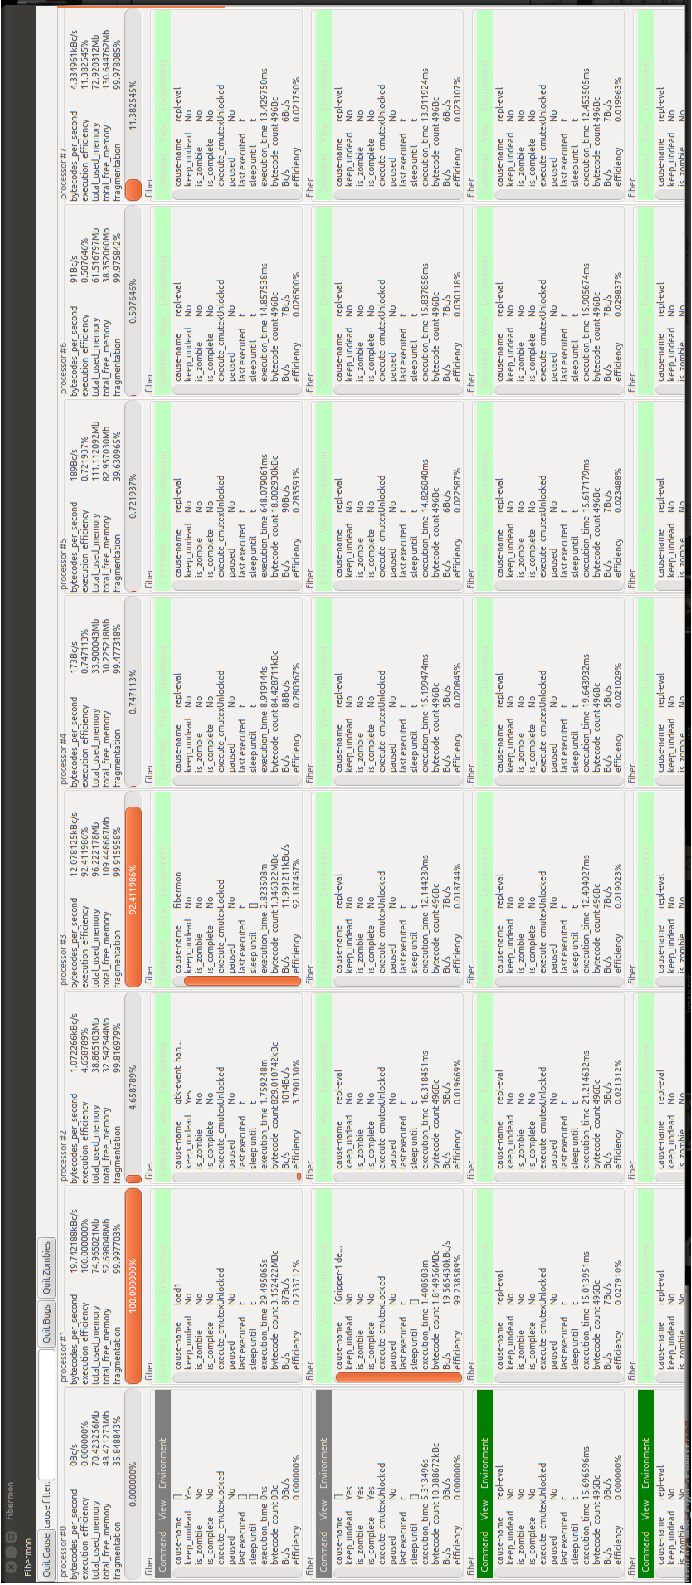
\includegraphics[width=10cm]{gfx/fibermon_many_fibers}
  \caption[FiberMon application monitoring many fibers]{FiberMon
    application monitoring hundreds of parallel fibers, simulated
    activities in Duration, executing on eight different physical
    processor cores.}
  \label{figure:fibermon_many_fibers}
\end{figure}

\section{Pausing and Resuming Activities}

SALS includes a {\tt pause} command to pause the current fiber:
\begin{equation*}
\text{\tt [pause]}
\end{equation*}
The {\tt pause} command causes the executing fiber to remove itself
from the scheduler, after removing itself, it yields the rest of the
scheduler cycle.  A fiber that is paused in this sense uses none of
SALS's processor resources because it is completely removed from
the scheduler.

If a fiber has paused, it cannot restart itself.  In order for a fiber
to resume execution, another executing fiber must use the
{\tt resume} command with the fiber object as an argument:
\begin{equation*}
\text{\tt [resume <fiber>]}
\end{equation*}

The {\tt pause} and {\tt resume} commands are extremely efficient for
managing large simulations in which most fibers will be inactive at
any given time, but they are a little cumbersome, so I have written a
lightweight and helpful \emph{fiber trigger} object, which I will
explain after explaining one more object that is used to program fiber
triggers.

\section{Mutual Exclusion}

SALS provides a primitive object called a \emph{mutex} for handling
the mutually exclusive access to resources.  A mutex object has two
possible states: locked and unlocked.  If the mutex object is unlocked
then when a fiber tries to locks the mutex, the mutex switches to the
locked state and the fiber continues execution.  If the mutex object
is already locked when a fiber tries to lock the mutex, the fiber will
pause until the mutex is unlocked, at which point the mutex will be
locked and the waiting fiber will resume execution.  Mutexes are used
for protecting shared resources from being used by more than one fiber
at a time.

Mutexes are a special type of object that must be supported by the
hardware of a concurrent computer.  Almost every parallel programming
language has a mutex construct that derives from this hardware mutex.
So, mutexes are common to parallel programming, but they are
notoriously difficult to debug, resulting in bugs affectionately
referred to as ``race conditions'' or ``deadlocks''.  In order to help
with debugging these types of problems, mutexes in SALS keep track of
which fibers are waiting for the lock or holding the lock.  I have
found this extra information invaluable in debugging complicated mutex
related bugs.

\section{Fiber Triggers}

The fiber trigger organizes sets of paused fibers so that they can be
woken up at the same time.  Basically, the fiber trigger is an object
that provides a useful abstraction for controlling fiber execution
that combines a mutex with the {\tt pause} and {\tt resume} commands.

A fiber can be added to the resume set of a fiber trigger by using the
{\tt wait-for-trigger} command as in the following example:
\begin{equation*}
\text{\tt [wait-for-trigger <fiber-trigger>]}
\end{equation*}
The {\tt wait-for-trigger} command atomically pauses the current fiber
and then adds the fiber to resume queue of the fiber trigger object.  The fiber trigger object provides a mutex object 

\section{leftovers...}

\section{Fiber Complete and Bug Found Triggers}

get fiber triggers from fiber objects.

execution complete versus bug found.


\section{{\tt par-fib}}

\begin{equation*}
\begin{array}{l}
\text{\tt [defunk par-fib [n]} \\
\text{\tt ~~[if [== n 0]} \\
\text{\tt ~~~~~~0} \\
\text{\tt ~~~~[if [== n 1]} \\
\text{\tt ~~~~~~~~1} \\
\text{\tt ~~~~~~[let [[x []]} \\
\text{\tt ~~~~~~~~~~~~[y []]]} \\
\text{\tt ~~~~~~~~[parog [= x [par-fib [- n 2]]]} \\
\text{\tt ~~~~~~~~~~~~~~~[= y [par-fib [- n 1]]]]} \\
\text{\tt ~~~~~~~~[+ x y]]]]]}
\end{array}
\end{equation*}


\section{Symbolic Statements in SALS}

\section{Three Categories of Symbol}

SALS programming expressions are combinations of symbols in lists.
It is important to keep all of these symbols straight.  I have so far
introduced three slightly different conceptions of symbols: (1) the
symbols that are reflectively symbolized from the activities of
Duration, (2) the symbols that a programmer types into a computer, and
(3) the simulated symbols that are generated by the simulated
first-order reflective layer of thinking.

\section{Concurrent Memory Allocation Pools}

SALS works off of a multiple pool memory allocation system that
allows separate pools for each concurrent virtual processor,
eliminating the need for many lock situations that occur with shared
memory pools.

\section{Garbage Collection}



\section{Layered Cognitive Architecture}

On this computational substrate, I have built a layered cognitive
architecture that is inspired by Minsky's description of the bottom
four layers of his Emotion Machine, or Model-6 architecture.  This
includes, a physical world, a reactive mapping of the physical world
to pre-symbolic activities, a first-order reflective thinking layer
that creates symbols, causal models, and plans for accomplishing
physical goals, as well as a second-order reflective thinking layer
that creates symbols, causal models, and plans for accomplishing
first-order thinking goals.  The theory behind this implementation
inductively explains how this implementation can be extended to an
arbitrary number of reflective thinking layers.  While this part of
the thesis is primarily focused on the simulation of an artificial,
modelled representation of this theory, I derive the fundamental basis
of my theory of mind in non-technical English in
\autoref{part:theory_of_mind}.

\section{Block Building Domain}

My architecture exists in three main theoretical parts: the physical
layer, the first-order reflective layer, and the second-order
reflective layer.  In order to explain how my theory allows for
learning at multiple levels, I use a simulation of a physical domain
that is easy to understand.  I use this simulation primarily for
communication of my working theory by demonstrating learning at
multiple reflective levels in response to a single physical failure.

My simulation of the physical block building domain is meant to appear
as similar to the canonical toy problem, \emph{Blocks World}, with one
key exception: my model is meant to have a different interpretation
than the original Blocks World.  The primary point to emphasize here
is that my physical simulation is meant to represent a dynamic
physical world as opposed to the logical and completely static
reference for the Blocks World physical domain.



\section{Reactive Layer}

The physical layer in my theory is implemented by combining the
physical simulation with a reactive layer that maps the physical
simulator perceptual and motor functions to ``sub-symbolic''
activities that are available to first-order reflection.



\section{Leftovers...}

\section{Data Reflection}



\section{The von Neumann Model}

\cite{von_neumann:1945} describes a model of computation that
introduces a concept called \emph{instructions} to the digital
abstraction.  Instructions are a predefined set of arrangements of
symbols that, with other data, determine the future arrangements of
symbols in memory.  Given the von Neumann model, the programming of
each new simulation can be done symbolically rather than by rewiring
the hardware every time.  The von Neumann model is a great technical
achievement that eases the manipulation of simulations, but
fundamentally, the same limitations of digital reflection exist for
the von Neumann model as exist for all computers.  This is because the
von Neumann model still assumes the static unchanging discrete
activity of the combinational device, which causes the transition from
the past to the future.  In the von Neumann model, the combinational
device is more complicated and allows the programmer to more easily
think more abstractly about programs as data.

\section{Instructional Reflection}

The von Neumann model introduces instruction sets that allow programs
to be stored in memory along with other data.

\section{Meaninglessness of the Digital Abstraction}



Because of the inability of a model based on the digital abstraction
to refer to the transition from the past to the future, a
computational model

\section{Leftovers...}

\section{Simulation of a Theory}

Creating a simulation of a theory of mind is useful for a variety of
reasons.  The primary use of simulation is to explore the mechanical
implications of different mechanical assumptions.

\section{Comparing Two Simulations}

Two simulations of two different theories is useful in finding
correlations between these theories.  In order for these correlations
to be meaningful, they must be contained within a more universal
theory that provides a reference to a universal reality.  The idea of
two realities is a contradiction in terms.


\section{Model-6}

My theory does not include Minsky's ``self-reflective'' or
``self-conscious'' layers.  I see objective models of self are
required for what Minsky discusses as self-reflective thinking,
including models of personality recognition and planning.  My model
does not yet have the capability to create or use subjective views of
objects, which I see as necessary not only for self-reflective
thinking, but also Minsky's concept of ``self-conscious'' thinking.
While singly recursive self-reflective statements, like ``Suzy wants
ice-cream'', require learning object and subject relationships, I see
doubly recursive descriptions of personality as necessary for Minsky's
conception of self-conscious thinking, e.g. ``Suzy wants Bob to want
ice-cream.''

